\section{Auswertung}
\subsection{Messung der Schallgeschwindigkeit}
Im ersten Teil des Versuchs soll die Schallgeschwindigkeit $c_{\symup{Acryl}}$ mit Hilfe der Ultraschallmessung bestimmt werden. Hierzu werden die zeitlichen
Abstände der Peaks der Reflektion gemessen und mit der Länge des Zylinders mit dem Weg-Zeit-Gesetz in Relation gesetzt
\begin{equation*}
  c_{\symup{Acryl}} = \frac{2l_1}{\symup\Delta t}
\end{equation*}
Die Messwerte und die berechnete Schallgeschwindigkeit für Acryl sind in Tabelle \ref{tab:1} aufgelistet. Die Messung der Peaks mit Verstärkung ist in
Abbildung \ref{abb:1} zu sehen.
\begin{table}
  \centering
  \caption{Messwerte zur Messung der Schallgeschwindigkeit von Acryl.}
  \label{tab:1}
  \begin{tabular}{c | c c | c c | c c}
    \toprule
    Länge des  & \multicolumn{2}{c|}{Peak 1} & \multicolumn{2}{c|}{Peak 1} & Zeitdifferenz & Schallgeschwindigkeit \\
    Zylinders $l_1$ / \si{\centi\meter} & $t_1$ / \si{\micro\second} & $U_1$ / \si{\volt} & $t_2$ / \si{\micro\second} & $U_2$ / \si{\volt} & \Delta $t$ /
     \si{\micro\second} & $c_{\symup{Acryl}} $ \si{\meter\per\second} \\
     \midrule
     \num{4,025(5)} & 30,4 & 1,300 & 60,0 & 0,139 & 29,6 & \num{2719,6(34)} \\
     \bottomrule
  \end{tabular}
\end{table}
\begin{figure}
  \centering
  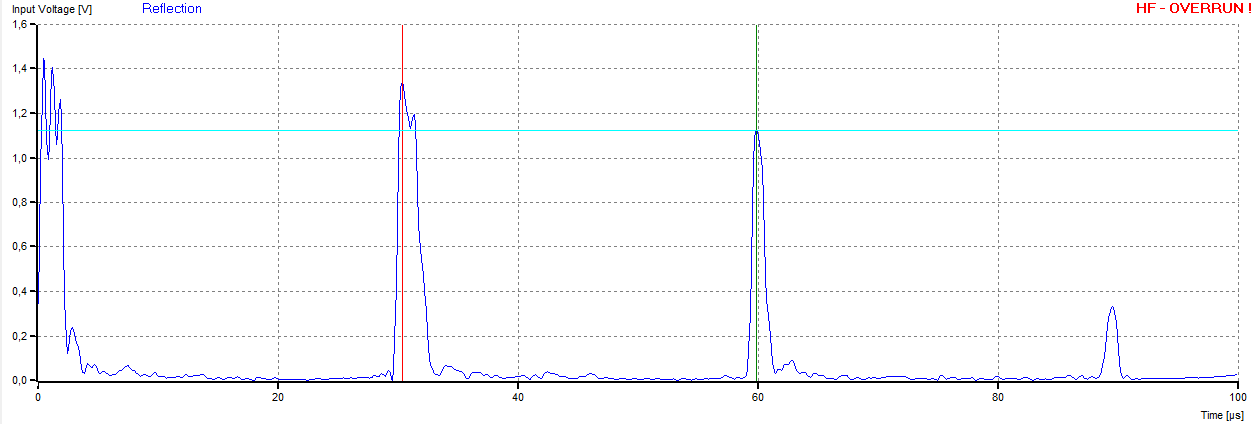
\includegraphics[scale=0.48]{Messung2.png}
  \caption{Messung der Schallgeschwindigkeit in Acryl (mit Verstärkung).}
  \label{abb:1}
\end{figure}

Mit Hilfe der berechneten Schallgeschwindigkeit kann nun die Länge des Zylinders mit einer Ultraschallsonde gemessen werden, indem die Schallgeschwindigkeit in
das Programm eingetragen wird und auf den Modus DEPTH umgestellt wird. Der entstehende Peak kann nun abgemessen werden, daraus folgt für die Länge des Zylinders
\begin{equation*}
  l_1 = \SI{4,13}{\centi\meter}
\end{equation*}

\subsection{Bestimmung der Dämpfung}
Bei der Berechnung der Dämpfung des Schalls wird die Eigenschaft der Proportionalität der gemessenen Spannung zur Intensität der Welle ausgenutzt, also
$I \propto U$. Aus den gemessenen Amplituden der reflektierten Ultraschallwelle und der Länge des Zylinders (siehe Tabelle \ref{tab:2}), wobei dieser
von dem Schall zwei mal durchlaufen wird, lässt sich eine exponentielle Regression der Form
\begin{equation*}
  U(l) = U_0 \exp(-\alpha l)
\end{equation*}
durchführen. Diese Regression liefert die Werte für $U_0$ und $\alpha$:
\begin{align*}
  U_0 &= \SI{3,0(8)}{\volt} \\
  \alpha &= \SI{11,5(28)}{\per\meter}
\end{align*}
\begin{table}
  \centering
  \caption{Messwerte zur Bestimmtung der Dämpfung, Impuls-Echo-Verfahren: Wobei $U$ die Spannung der reflektierten Welle ist und $l$ die Länge des Zylinders.}
  \label{tab:2}
  \begin{tabular}{c c}
    \toprule
    $U$ / \si{\volt} & $l$ / \si{\centi\meter} \\
    \midrule
     1,367 & 4,025 \\
     0,055 & 12,05 \\
     0,645 & 6,16 \\
     1,300 & 3,10 \\
     0,063 & 10,20 \\
     0,412 & 8,04 \\
     0,928 & 7,08  \\
    \bottomrule
  \end{tabular}
\end{table}
\begin{figure}
  \centering
  \includegraphics[scale=0.7]{PlotDämpfung.pdf}
  \caption{Exponentielle Regression derDämpfung, Impuls-Echo-Verfahren.}
  \label{abb:2}
\end{figure}

\subsection{Messung der Schallgeschwindigkeit mit dem Impuls-Echo-Verfahren}
Zur Messung der Schallgeschwindigkeit mittels Impuls-Echo-Verfahren wird aufgrund systematischer eine lineare Regression der Form
\begin{equation*}
  \frac{t}{2} = l \cdot c_1 -l_{0,1}
\end{equation*}
durchgeführt, wobei $l$ die Länge des Zylinderns, $c_1$ die Schallgeschwindigkeit, $l_{0,1}$ die Dicke der Grenzschicht und $t$ die zurückgelegte Zeit der
Ultraschallwellen beschreibt.
Diese Regression liefert die Werte für $c_1$ und $l_{0,1}$:
\begin{align*}
  c_1 &= \SI{2727(21)}{\meter\per\second} \\
  l_{0,1} &= \SI{0,7(6)}{\milli\meter}
\end{align*}
Die Messwerte sind in Tabelle \ref{tab:2} aufgelistet und mit der Regression in Abbildung \ref{abb:3} dargestellt.
Bei der Berechnung der Regression wurde ein stark abweichender Messwert nicht mit einbezogen, da der Zylinder bei der Messung durch zwei kleinere Zylinder
zusammengesetzt wurde und deswegen die Grenzschicht aus Wasser zwischen den Zylindern zu starken Fehlern in der Berechnung führt.
\begin{figure}
  \centering
  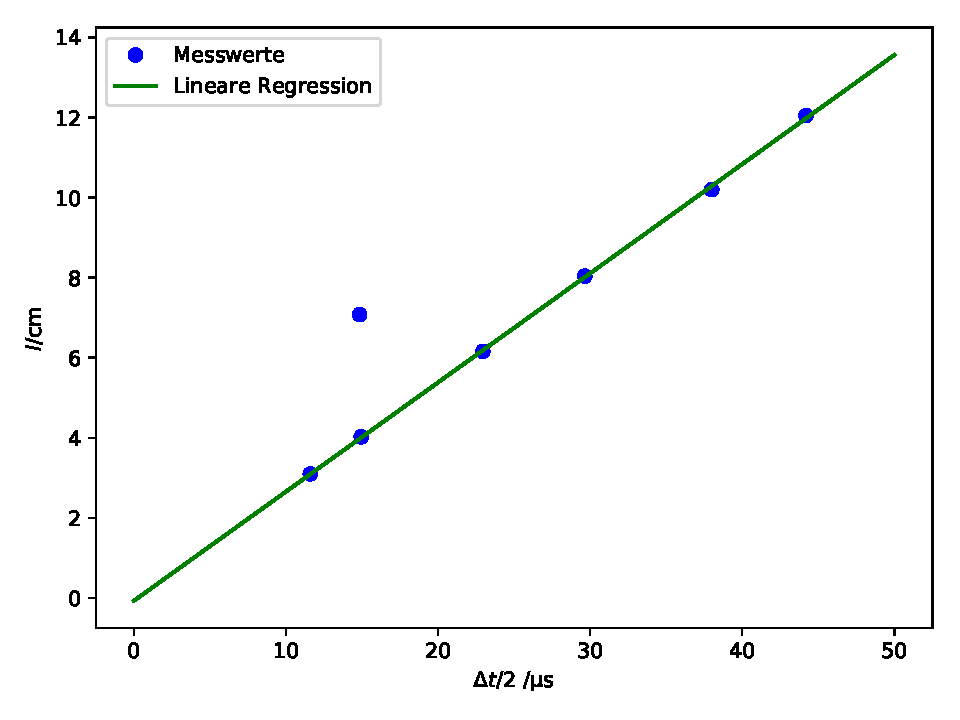
\includegraphics[scale=0.7]{Schallgeschwindigkeit1.pdf}
  \caption{Messung der Schallgeschwindigkeit mittels Impuls-Echo-Verfahren.}
  \label{abb:3}
\end{figure}

\subsection{Messung der Schallgeschwindigkeit mit dem Durchschallungsverfahren}
Die Berechnung der Schallgeschwindigkeit mittels des Durchschallungsverfahren ist ähnlich, wie die des Impuls-Echo-Verfahrens. Der einzige Unterschied ist hierbei
die Zeit, da der Schall nur einmal durch den Zyliner geht, muss hier nicht die halbe Zeit genommen werden.
Es wird also eine lineare Regression der Form
\begin{equation*}
  t = l \cdot c_2 -l_{0,2}
\end{equation*}
durchgeführt, wobei $l$ die Länge des Zylinders, $c_2$ die Schallgeschwindigkeit, $l_{0,2}$ die Dicke der Grenzschicht und $t$ die Zeit beschreibt, die
der Schall durch das Medium benötigt. Diese Regression liefert die Werte
\begin{align*}
  c_2 &= \SI{2711(30)}{\meter\per\second} \\
  l_{0,1} &= \SI{2,4(9)}{\milli\meter}
\end{align*}
Die Messwerte und die Regression sind in \ref{abb:4} abgebildet. Die Messwerte sind in Tabelle \ref{tab:3} aufgelistet.
\begin{table}
  \centering
  \caption{Messwerte zur Messung der Schallgeschwindkeit mittels Durchschallungsverfahren.}
  \label{tab:3}
  \begin{tabular}{c c}
    \toprule
    $t$ / \si{\micro\second} & $l$ / \si{\centi\meter} \\
    \midrule
    12,6  &  3,1 \\
    15,4  &  4,025 \\
    30,5  &  8,04 \\
    38,9  &  10,20 \\
    45,1  &  12,05 \\
    23,6  &  6,16 \\
    \bottomrule
  \end{tabular}
\end{table}
\begin{figure}
  \centering
  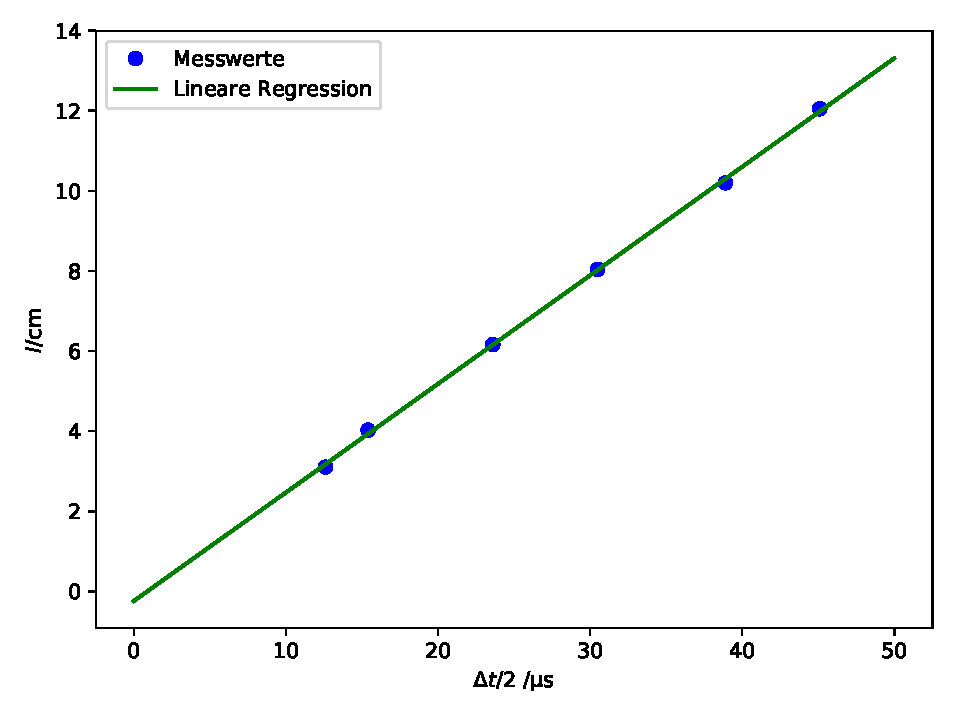
\includegraphics[scale=0.7]{Schallgeschwindigkeit.pdf}
  \caption{Messung der Schallgeschwindigkeit mittels Durchschallungsverfahren.}
  \label{abb:4}
\end{figure}

\subsection{Spektrale Analyse und Cepstrum}
Zur Messung der Dicke der Platten wird die Schallgeschwindigkeit der Messung am Anfang eingestellt und in den Modus Depth umgeschaltet. Hierbei wird direkt
die Dicke ausgemessen, indem die Differenz der Peaks gemessen wird. Für die Dicke der Platten ergibt sich
\begin{align*}
  d_1 = \SI{0,61}{\centi\meter} \\
  d_2 = \SI{1,15}{\centi\meter}
\end{align*}

\begin{table}
  \centering
  \caption{Messwerte zur Bestimmung der Dicke der Acrylplatten.}
  \label{tab:4}
  \begin{tabular}{c c c c}
    \toprule
    & Peak 1 & Peak 2 & Dicke \\
    & $d_1$ / \si{\milli\meter} & $d_2$ / \si{\milli\meter} & $d$ / \si{\milli\meter} \\
    \midrule
    Zylinder & 0,6 & 40,9 & 40,3 \\
    Platte 1 & 40,9 & 47,0 & 6,1 \\
    Platte 2 & 47,0 & 58,5 & 11,5 \\
    \bottomrule
  \end{tabular}
\end{table}

Außerdem wird für diesen Versuchsteil ein FFT (Fast-Fourier-Transformation) durchgeführt. Dieses spaltet das enstandene Spektrum in
ein Frequenzspektrum auf. Das Cepstrum ist in Abbildung \ref{abb:5} zu sehen.
\begin{figure}
  \centering
  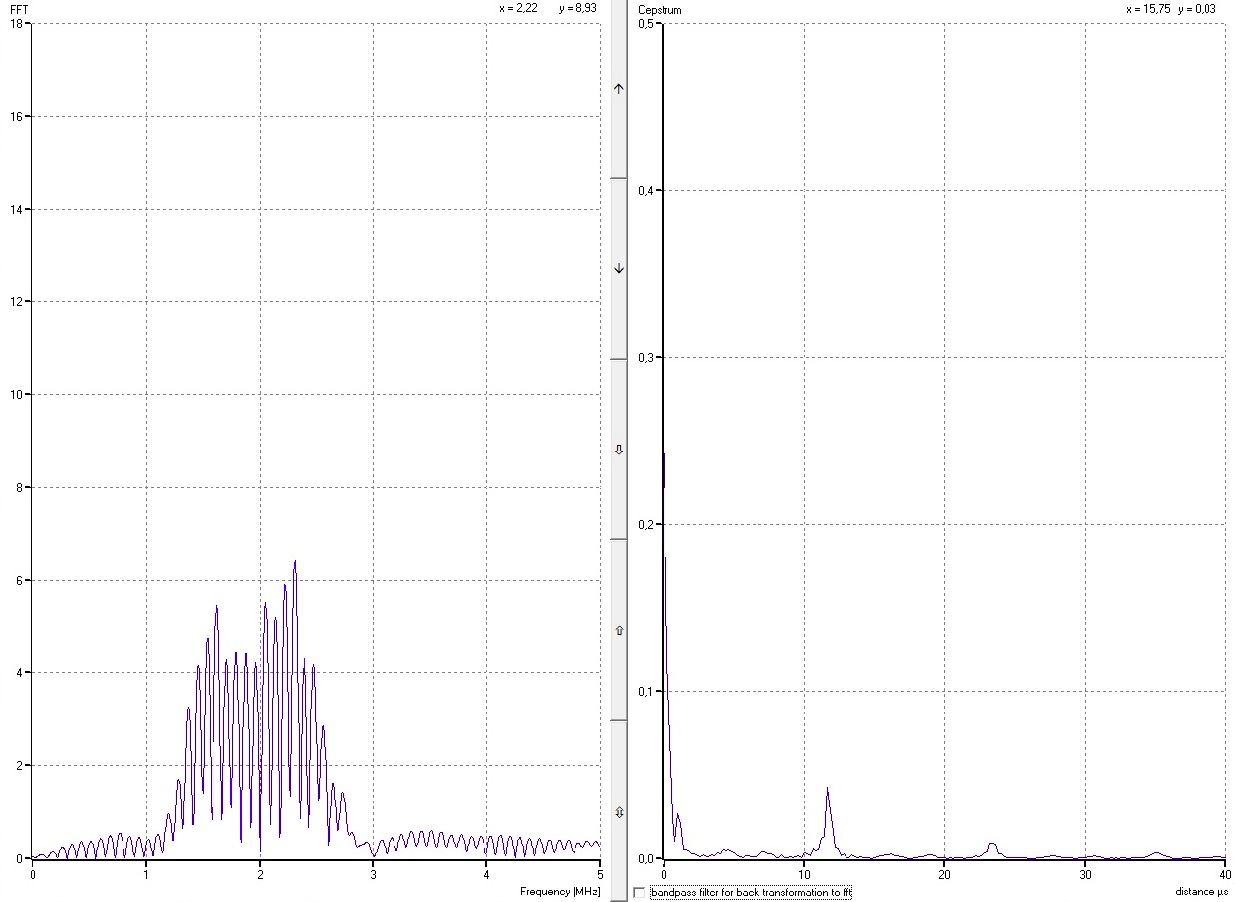
\includegraphics[scale=0.3]{Cepstrum.png}
  \caption{Cepstrum.}
  \label{abb:5}
\end{figure}

\subsection{Ausmessung des Augenmodels mittels Impuls-Echo-Verfahren}
Zur Vermessung des Augenmodels werden die Zeiten $t$ berechnet, die der Schall durch den jeweiligen Bereich benötigt. Hierbei muss beachtet werden, dass erneut
das Impuls-Echo-Verfahren verwendet wird und der Schall durch die Reflektion zweimal durch den jeweiligen Bereich läuft, deswegen muss die berechnete Zeit halbiert werden.
Die Schallgeschwindigkeit in der Glaskörperflüssigkeit beträgt $c_{\symup{GK}}=\SI{1410}{\meter\per\second}$ und in der Linse
$c_{\symup{L}}=\SI{2500}{\meter\per\second}$ \cite{Q1}.
Die aus dem Diagramm \ref{abb:6} abgelesenen Werte sind in Tabelle \ref{tab:5} aufgelistet. Aus diesen Werte folgt für den Bereich von der Hornhaut bis zur Iris:
\begin{align*}
  \Delta t_1 =& \SI{10,9}{\micro\second} \\
  l_1 =& \Delta t_1 \cdot c_{\symup{GK}} = \SI{7,68}{\milli\meter}
\end{align*}
Der Abstand zwischen der Iris und der Linse:
\begin{align*}
  \Delta t_2 =& \SI{5,8}{\micro\second} \\
  l_2 =& \Delta t_2 \cdot c_{\symup{GK}} = \SI{4,09}{\milli\meter}
\end{align*}
Der Dicke der Linse:
\begin{align*}
  \Delta t_3 =& \SI{6,5}{\micro\second} \\
  l_3 =& \Delta t_3 \cdot c_{\symup{L}} = \SI{8,13}{\milli\meter}
\end{align*}
und die Dicke des Glaskörpers:
\begin{align*}
  \Delta t_4 =& \SI{48,6}{\micro\second} \\
  l_4 =& \Delta t_4 \cdot c_{\symup{GK}} = \SI{34,97}{\milli\meter}
\end{align*}

\begin{figure}
  \centering
  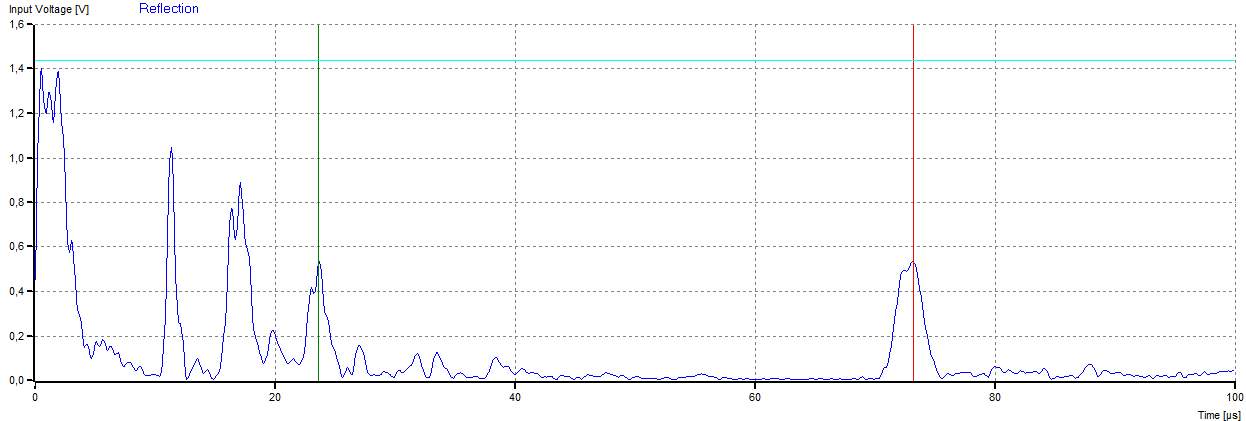
\includegraphics[scale=0.4]{Auge_Zeit.png}
  \caption{Vermessung des Auges mittels Impuls-Echo-Verfahren.}
  \label{abb:6}
\end{figure}

\begin{table}
  \centering
  \caption{Daten zur Vermessung des Auges.}
  \label{tab:5}
  \begin{tabular}{c c}
    \toprule
    Amplitude & Zeit \\
    & $t$ / \si{\micro\second} \\
    \midrule
    A1 & 0,4 \\
    A2 & 11,3 \\
    A3 & 17,1 \\
    A4 & 23,6 \\
    A5 & 73,2 \\
    \bottomrule
  \end{tabular}
\end{table}

\section{Diskussion}

Im ersten Versuchsteil wurde der Zylinder einmal mit der Schieblehre und einmal per Impuls-Echo-Verfahren ausgemessen.
Hierbei entstanden Unterschiede von bis zu \SI{1,83}{\percent}.
\begin{table}
  \centering
  \caption{Messung des Zylinders.}
  \label{d:tab:1}
  \begin{tabular}{c c c}
    \toprule
    Schieblehre & Impuls-Echo-Verfahren & Abweichung \\
    $l_1$ / \si{\milli\meter} & $l_1$ / \si{\milli\meter} & $p$ / \si{\percent} \\
    \midrule
    \num{40,25(5)} & 41,3 & 1,83 \\
    \bottomrule
  \end{tabular}
\end{table}

Außerdem wurde bei dem Versuchsteil zur Messung der Schallgeschwindigkeit ein Acrylzylinder verwendet, der aus zwei einzelnen mittels einer Wasserschicht
zusammengesetzt wurde. Dies führt zu Verfälschungen der Messung, da der Schall eine kurze Strecke durch Wasser hindurch muss und für diese Strecke eine
andere Schallgeschwindigkeit besitzt. Dieser Fehler wurde aber soweit minimiert, dass der entsprechende Wert für die Regression herausgenommen wurde.
Dennoch wurde ein Fehler von maximal \SI{0,7}{\percent} gemessen.
\begin{table}
  \centering
  \caption{Messung des Zylinders.}
  \label{d:tab:2}
  \begin{tabular}{c| c c|  c c}
    \toprule
    Literaturwert & Impuls-Echo- & Abweichung & Durchschallungs- & Abweichung \\
    & Verfahren & (IEV) & verfahren & (DSV) \\
    $c$ / \si{\meter\per\second} & $c_{\symup{IEV}}$ / \si{\meter\per\second} & $p_{\symup{IEV}}$ / \si{\percent} & $c_{\symup{DSV}}$ / \si{\meter\per\second} & $p_{\symup{DSV}}$ / \si{\percent}\\
    \midrule
    2730 & \num{2727(21)} & 0,11 & 2711(30) & 0,70 \\
    \bottomrule
  \end{tabular}
\end{table}

\nocite{*}
\printbibliography
